\documentclass[aspectratio=169,12pt]{beamer}
\usepackage[utf8]{inputenc}
\usepackage{amsmath, amssymb}
\usepackage{booktabs}
\usepackage{hyperref}
\usepackage{listings}
\usepackage{tikz}
\usetheme{Madrid}
% Show slide number as "current/total" in the footer
\setbeamertemplate{footline}{%
  \leavevmode\hbox{\begin{beamercolorbox}[wd=\paperwidth,ht=2.25ex,dp=1ex,center]{author in head/foot}%
    \usebeamerfont{author in head/foot}\insertframenumber/\inserttotalframenumber
  \end{beamercolorbox}}%
  \vskip0pt%
}
\setbeamertemplate{navigation symbols}{}

\title{Computer Structure -- Cache Memory}
\author{Based on slides by Lihu Rappoport}
\date{Technion CSL}

\begin{document}

\begin{frame}
  \titlepage
\end{frame}

% --- Overview
\begin{frame}{Processor--Memory Gap (summary)}
\begin{itemize}
  \item CPU performance has improved much faster than DRAM latency/bandwidth.
  \item The performance gap has grown roughly $\sim 50\%$/year historically.
  \item Motivation: hide long memory access times from the CPU.
\end{itemize}
\end{frame}

\begin{frame}{Memory Trade-Offs}
\begin{itemize}
  \item Large (dense) memories are \textbf{slow}
  \item Fast memories are \textbf{small}, expensive and consume high power
  \item Goal: give the processor a feeling that it has a memory which is large (dense), fast, consumes low power, and cheap
  \item Solution: a Hierarchy of memories
\end{itemize}

\vspace{0.3cm}
\begin{center}
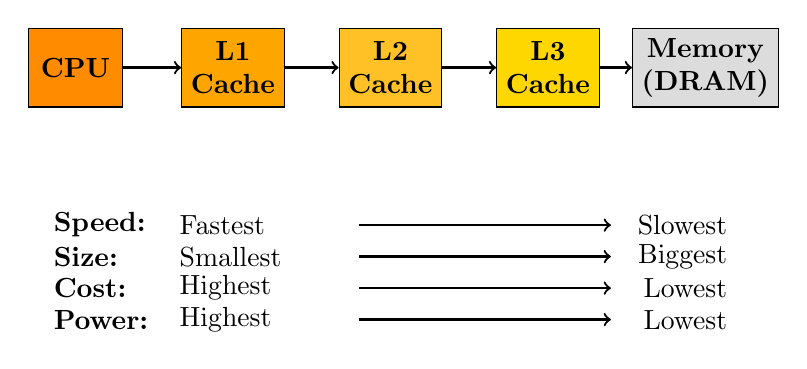
\begin{tikzpicture}[scale=0.8]
  % Define colors for the hierarchy
  \definecolor{cpucolor}{RGB}{255,140,0}      % Orange
  \definecolor{l1color}{RGB}{255,165,0}       % Orange
  \definecolor{l2color}{RGB}{255,193,37}      % Yellow-orange
  \definecolor{l3color}{RGB}{255,215,0}       % Gold
  \definecolor{memcolor}{RGB}{220,220,220}    % Light gray
  
  % Memory hierarchy boxes
  \node[rectangle, draw, fill=cpucolor, minimum width=1.2cm, minimum height=1cm, align=center, font=\bfseries] (cpu) at (0,0) {CPU};
  \node[rectangle, draw, fill=l1color, minimum width=1.2cm, minimum height=1cm, align=center, font=\bfseries] (l1) at (2.5,0) {L1\\Cache};
  \node[rectangle, draw, fill=l2color, minimum width=1.2cm, minimum height=1cm, align=center, font=\bfseries] (l2) at (5,0) {L2\\Cache};
  \node[rectangle, draw, fill=l3color, minimum width=1.2cm, minimum height=1cm, align=center, font=\bfseries] (l3) at (7.5,0) {L3\\Cache};
  \node[rectangle, draw, fill=memcolor, minimum width=1.2cm, minimum height=1cm, align=center, font=\bfseries] (mem) at (10,0) {Memory\\(DRAM)};
  
  % Arrows between boxes
  \draw[->, thick] (cpu.east) -- (l1.west);
  \draw[->, thick] (l1.east) -- (l2.west);
  \draw[->, thick] (l2.east) -- (l3.west);
  \draw[->, thick] (l3.east) -- (mem.west);
  
  % Characteristics table below
  \node[anchor=west, font=\bfseries] at (-0.5,-2.5) {Speed:};
  \node[anchor=west] at (1.5,-2.5) {Fastest};
  \draw[->, thick] (4.5,-2.5) -- (8.5,-2.5);
  \node[anchor=east] at (10.5,-2.5) {Slowest};
  
  \node[anchor=west, font=\bfseries] at (-0.5,-3) {Size:};
  \node[anchor=west] at (1.5,-3) {Smallest};
  \draw[->, thick] (4.5,-3) -- (8.5,-3);
  \node[anchor=east] at (10.5,-3) {Biggest};
  
  \node[anchor=west, font=\bfseries] at (-0.5,-3.5) {Cost:};
  \node[anchor=west] at (1.5,-3.5) {Highest};
  \draw[->, thick] (4.5,-3.5) -- (8.5,-3.5);
  \node[anchor=east] at (10.5,-3.5) {Lowest};
  
  \node[anchor=west, font=\bfseries] at (-0.5,-4) {Power:};
  \node[anchor=west] at (1.5,-4) {Highest};
  \draw[->, thick] (4.5,-4) -- (8.5,-4);
  \node[anchor=east] at (10.5,-4) {Lowest};
\end{tikzpicture}
\end{center}
\end{frame}

\begin{frame}{Why Hierarchy Works}
\begin{itemize}
  \item \textbf{Temporal Locality (Locality in Time):}
  \begin{itemize}
    \item If an item is referenced, it will tend to be referenced again soon
    \item Example: code and variables in loops
  \end{itemize}
  $\Rightarrow$ \textbf{Keep recently accessed data closer to the processor}
  
  \vspace{0.5cm}
  
  \item \textbf{Spatial Locality (Locality in Space):}
  \begin{itemize}
    \item If an item is referenced, nearby items tend to be referenced soon
    \item Example: scanning an array
  \end{itemize}
  $\Rightarrow$ \textbf{Move contiguous blocks closer to the processor}
  
  \vspace{0.5cm}
  
  \item \textbf{Locality + smaller HW is faster + Amdahl's law}\\
  $\Rightarrow$ \textbf{memory hierarchy}
\end{itemize}
\end{frame}

\begin{frame}{Memory Hierarchy: Terminology}
\begin{itemize}
  \item \textbf{For each memory level define the following}
  \begin{itemize}
    \item \textcolor{green!60!black}{\textbf{Hit:}} data of the requested address is available in the cache level
    \item \textcolor{green!60!black}{\textbf{Miss:}} data of the requested address is not available in the cache level
    \item \textcolor{green!60!black}{\textbf{Hit Rate:}} the fraction of accesses that hit in that cache level
    \begin{itemize}
      \item For L1 cache: \#L1 hits / \#data accesses in the program
      \item For L2 cache: \#L2 hits / \#L1 misses
    \end{itemize}
    \item \textcolor{green!60!black}{\textbf{Hit Time:}} time from data request till data received when hitting in the cache level; includes the time to determine hit/miss
    \item \textcolor{green!60!black}{\textbf{Miss Rate}} = $1 - (\text{Hit Rate})$
    \item \textcolor{green!60!black}{\textbf{Miss Penalty:}} Time to replace a block in the upper level + Time to deliver the block the processor
  \end{itemize}
  
  \vspace{0.3cm}
  
  \item \textbf{Average memory-access time =}\\
  \hspace{1cm} $t_{\text{effective}} = (\text{Hit time} \times \text{Hit Rate}) + (\text{Miss Time} \times \text{Miss rate})$\\
  \hspace{2.2cm} $= (\text{Hit time} \times \text{Hit Rate}) + (\text{Miss Time} \times (1-\text{Hit rate}))$
  \begin{itemize}
    \item If hit rate is close to 1, $t_{\text{effective}}$ is close to Hit time
  \end{itemize}
\end{itemize}
\end{frame}

\begin{frame}{Effective Memory Access Time}
\begin{itemize}
  \item \textbf{Cache -- holds a subset of the memory}
  \begin{itemize}
    \item Hopefully -- the subset being used now
  \end{itemize}
  
  \item \textbf{Effective memory access time}
  \begin{itemize}
    \item $t_{\text{effective}} = (t_{\text{cache}} \times \text{Hit Rate}) + (t_{\text{mem}} \times (1 - \text{Hit rate}))$
    \item $t_{\text{mem}}$ includes the time it takes to detect a cache miss
  \end{itemize}
  
  \item \textbf{Example}
  \begin{itemize}
    \item Assume $t_{\text{cache}} = 10$ nsec and $t_{\text{mem}} = 100$ nsec
  \end{itemize}
\end{itemize}

\begin{center}
\begin{tabular}{c|c|l}
\textbf{Hit Rate} & \textbf{$t_{\text{eff}}$ (nsec)} & \textbf{Computation} \\
\hline
0 & 100 & $(0.0 \times 10) + (1.0 \times 100)$ \\
50 & 55 & $(0.5 \times 10) + (0.5 \times 100)$ \\
90 & 19 & $(0.9 \times 10) + (0.1 \times 100)$ \\
99 & 10.9 & $(0.99 \times 10) + (0.01 \times 100)$ \\
99.9 & 10.1 & $(0.999 \times 10) + (0.001 \times 100)$ \\
\end{tabular}
\end{center}

\begin{itemize}
  \item $t_{\text{mem}}/t_{\text{cache}}$ goes up $\Rightarrow$ more important that hit-rate closer to 1
\end{itemize}
\end{frame}

\begin{frame}{Cache -- Main Idea}
\begin{columns}[T]
\begin{column}{0.65\textwidth}
\begin{itemize}
  \item \textcolor{blue}{\textbf{The cache holds a small part of the entire memory}}
  \begin{itemize}
    \item Need to map parts of the memory into the cache
  \end{itemize}
  
  \item \textcolor{blue}{\textbf{Main memory is (logically) partitioned into blocks}}
  \begin{itemize}
    \item Typical block size is 32 or 64 bytes
    \item Blocks are aligned
  \end{itemize}
  
  \item \textcolor{blue}{\textbf{The cache partitioned into cache lines}}
  \begin{itemize}
    \item Each cache line holds a memory block
    \item Only a subset of the memory blocks are mapped to the cache at a given time
    \item The cache views an address as
  \end{itemize}
\end{itemize}

\vspace{0.3cm}
% Address format at the bottom of text
\begin{center}
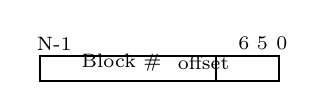
\begin{tikzpicture}[scale=0.8]
  \node[anchor=west, font=\scriptsize] at (0, 0.3) {N-1};
  \node[anchor=center, font=\scriptsize] at (1.5, 0) {Block \#};
  \node[anchor=center, font=\scriptsize] at (2.8, 0) {offset};
  \node[anchor=west, font=\scriptsize] at (3.2, 0.3) {6 5};
  \node[anchor=west, font=\scriptsize] at (3.8, 0.3) {0};
  
  % Address format boxes
  \draw[thick] (0.2, 0.1) rectangle (3.0, -0.3);
  \draw[thick] (3.0, 0.1) rectangle (4.0, -0.3);
\end{tikzpicture}
\end{center}
\end{column}

\begin{column}{0.35\textwidth}
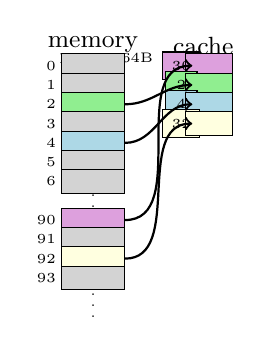
\begin{tikzpicture}[scale=0.7]
  % Define colors
  \definecolor{lightblue}{RGB}{173,216,230}
  \definecolor{lightgreen}{RGB}{144,238,144}
  \definecolor{lightyellow}{RGB}{255,255,224}
  \definecolor{lightpurple}{RGB}{221,160,221}
  \definecolor{lightgray}{RGB}{211,211,211}
  
  % Memory column
  \node[anchor=north, font=\bfseries, font=\small] at (1.2, 4.5) {memory};
  \node[anchor=north, font=\tiny] at (1.2, 4.2) {Block \#};
  \node[anchor=north, font=\tiny] at (2.0, 4.2) {64B};
  
  % Memory blocks with block numbers on the left
  \foreach \i/\color in {0/lightgray, 1/lightgray, 2/lightgreen, 3/lightgray, 4/lightblue, 5/lightgray, 6/lightgray} {
    \node[font=\tiny, anchor=east] at (0.7, 3.8-\i*0.35) {\i};
    \node[rectangle, draw, minimum width=0.8cm, minimum height=0.3cm, fill=\color] (mem\i) at (1.2, 3.8-\i*0.35) {};
  }
  
  % Dots for continuation
  \node[font=\tiny] at (1.2, 1.4) {\vdots};
  
  % More memory blocks
  \foreach \i/\color in {90/lightpurple, 91/lightgray, 92/lightyellow, 93/lightgray} {
    \pgfmathsetmacro{\ypos}{1.0-(\i-90)*0.35}
    \node[font=\tiny, anchor=east] at (0.7, \ypos) {\i};
    \node[rectangle, draw, minimum width=0.8cm, minimum height=0.3cm, fill=\color] (mem\i) at (1.2, \ypos) {};
  }
  
  % More dots
  \node[font=\tiny] at (1.2, -0.4) {\vdots};
  
  % Cache column
  \node[anchor=north, font=\bfseries, font=\small] at (3.2, 4.5) {cache};
  
  % Cache blocks split into tag and data - no spacing between boxes
  \foreach \tag/\color/\ypos in {30/lightpurple/3.8, 2/lightgreen/3.45, 4/lightblue/3.1, 32/lightyellow/2.75} {
    % Tag part (left)
    \node[rectangle, draw, minimum width=0.4cm, minimum height=0.3cm, fill=\color, font=\tiny] at (2.8, \ypos) {\tag};
    % Data part (right)
    \node[rectangle, draw, minimum width=0.6cm, minimum height=0.3cm, fill=\color] (cache\ypos) at (3.3, \ypos) {};
  }
  
  % Arrows from memory to cache
  \draw[->, thick] (mem2.east) to[out=0, in=180] (3.0, 3.45);
  \draw[->, thick] (mem4.east) to[out=0, in=180] (3.0, 3.1);
  \draw[->, thick] (mem90.east) to[out=0, in=180] (3.0, 3.8);
  \draw[->, thick] (mem92.east) to[out=0, in=180] (3.0, 2.75);
  
\end{tikzpicture}
\end{column}
\end{columns}
\end{frame}

\begin{frame}{Cache Lookup (summary)}
\begin{itemize}
  \item \textbf{Hit}: return data using the block offset.
  \item \textbf{Miss}: perform a \textbf{line fill} (may require several bus cycles).
  \item May need to \textbf{evict} another block to make room.
\end{itemize}
\end{frame}

\begin{frame}{Fully Associative (FA) Cache}
\begin{itemize}
  \item Any block can map to any line; tags of all lines are compared in parallel.
  \item Pros: lowest conflict misses. Cons: many comparators (area/power).
  \item On a tag match, return data using the offset.
\end{itemize}
\end{frame}

\begin{frame}{Valid Bit}
\begin{itemize}
  \item Cache starts empty; each line needs a \textbf{valid} bit.
  \item Valid set on fill; lines may be invalidated later.
\end{itemize}
\end{frame}

\begin{frame}{Direct-Mapped (DM) Cache}
\begin{itemize}
  \item Block number $\rightarrow$ \textbf{set} (index) + \textbf{tag}.
  \item Each block maps to exactly \emph{one} line: single comparator.
  \item Pros: simple, low power, fast. Cons: more \textbf{conflict} misses.
\end{itemize}
\end{frame}

\begin{frame}{2-Way Set Associative (2W SA)}
\begin{itemize}
  \item Each set holds 2 lines (ways); a block can reside in either way of its set.
  \item Requires two tag comparisons + way mux; fewer conflict misses than DM.
  \item Cache size $=\#\text{ways}\times\#\text{sets}\times\text{block size}$.
\end{itemize}
\end{frame}

\begin{frame}{Replacement Policies}
\begin{itemize}
  \item DM: victim is forced (the indexed line).
  \item N-way SA: choose victim among the ways in the set.
  \item Algorithms: \textbf{Optimal} (theoretical), \textbf{FIFO}, \textbf{Random}, \textbf{LRU}.
  \item LRU tends to perform best, but often only slightly better than Random.
\end{itemize}
\end{frame}

\begin{frame}[fragile]{LRU Implementation (sketch)}
\begin{itemize}
  \item 2-way: keep 1 bit per set indicating most recently used way.
  \item $k$-way: maintain per-set way-order counters (costly to update).
\end{itemize}
\begin{block}{Pseudo-code (on access of way $i$)}
\begin{lstlisting}[basicstyle=\ttfamily\small]
X = Counter[i]
Counter[i] = k-1          // way i becomes MRU
for j in [0..k-1]:
  if j != i and Counter[j] > X: Counter[j]--
\end{lstlisting}
Evict the way whose counter is 0.
\end{block}
\end{frame}

\begin{frame}{Pseudo-LRU (PLRU) Idea}
\begin{itemize}
  \item Use a binary-tree of $n-1$ bits for $n$ ways to track a \emph{partial} order.
  \item Update bits to point toward the accessed leaf; choose victim by walking opposite.
  \item Cheaper than true LRU; not always picks the true LRU way.
\end{itemize}
\end{frame}

\begin{frame}{Cache Line Size Trade-offs}
\begin{itemize}
  \item Larger lines exploit spatial locality but may fetch unused data $\rightarrow$ more evictions.
  \item Larger lines increase \textbf{miss penalty}; ``critical word first'' helps.
  \item $t_{\text{avg}} = t_{hit}\cdot(1-\text{MR}) + t_{miss}\cdot \text{MR}$.
\end{itemize}
\end{frame}

\begin{frame}{Performance Impact}
\begin{itemize}
  \item \textbf{MPI} (misses per instruction) = misses/access $\times$ accesses/instr.
  \item Memory stall cycles $= \text{IC}\cdot \text{MPI}\cdot \text{miss penalty}$.
  \item CPU time $= \text{IC}\cdot(\text{CPI}_{exec}+\text{MPI}\cdot \text{miss penalty})\cdot \text{cycle time}$.
\end{itemize}
\end{frame}

\begin{frame}{Classifying Misses: The 3Cs}
\begin{itemize}
  \item \textbf{Compulsory}: first reference to a block $\Rightarrow$ prefetch to mitigate.
  \item \textbf{Capacity}: working set $>$ cache size $\Rightarrow$ increase size / stream buffers.
  \item \textbf{Conflict}: set mapping causes evictions $\Rightarrow$ higher associativity / victim cache.
\end{itemize}
\end{frame}

\begin{frame}{Line Fill and Fill Buffers}
\begin{itemize}
  \item Missed block arrives in chunks; critical-chunk-first to reduce latency.
  \item Fill buffer accumulates full line, then writes to cache; also searched on access.
  \item ``Streaming'' loads may bypass L1 fill to avoid pollution.
\end{itemize}
\end{frame}

\begin{frame}{Victim Cache}
\begin{itemize}
  \item Small FA cache that holds lines evicted from L1.
  \item Checked in parallel with L1; on hit, swap victim back to L1.
  \item Reduces conflict pressure, especially for direct-mapped L1.
\end{itemize}
\end{frame}

\begin{frame}{Memory Updates on Writes}
\begin{columns}[T]
\column{0.5\textwidth}
\textbf{Write-back}
\begin{itemize}
  \item Write hits update only cache; line marked \emph{dirty}.
  \item Evict: write entire line to next level.
\end{itemize}
\column{0.5\textwidth}
\textbf{Write-through}
\begin{itemize}
  \item Write hits update cache \emph{and} next level.
  \item Needs a write buffer; evictions are clean.
\end{itemize}
\end{columns}
\end{frame}

\begin{frame}{Write Buffer \& Write Combining}
\begin{itemize}
  \item Buffer decouples CPU stores from DRAM writes.
  \item Combine multiple writes to same line into one buffer entry.
  \item On a miss, also consult write buffer for the most up-to-date bytes.
\end{itemize}
\end{frame}

\begin{frame}{Cache Write Miss Policies}
\begin{itemize}
  \item \textbf{Write-allocate}: fetch line on a store-miss (pairs with write-back).
  \item \textbf{No-write-allocate}: write directly to memory (pairs with write-through).
\end{itemize}
\end{frame}

\begin{frame}{Prefetching}
\begin{itemize}
  \item \textbf{HW prefetch}: next-line/streaming, stride, and more general pattern detectors.
  \item \textbf{SW prefetch}: explicit instructions (non-faulting hints).
  \item Aggressiveness must be tuned; over-prefetching wastes bandwidth and pollutes caches.
\end{itemize}
\end{frame}

\begin{frame}{Code Optimizations for Locality}
\begin{itemize}
  \item \textbf{Merging arrays}: AoS vs SoA trade-offs; reduce conflicts, improve spatial locality.
  \item \textbf{Loop fusion}: combine loops with same traversal to increase reuse.
  \item \textbf{Loop interchange}: access arrays in memory order to exploit spatial locality.
\end{itemize}
\end{frame}

\begin{frame}{Improving Cache Performance (summary)}
\begin{itemize}
  \item \textbf{Reduce miss rate}: bigger caches/lines, higher associativity, victim cache, stream buffers, prefetching, compiler transforms.
  \item \textbf{Reduce miss penalty}: early restart/critical word first, non-blocking caches, L2/L3.
  \item \textbf{Reduce hit time}: smaller, on-chip, direct-mapped L1.
\end{itemize}
\end{frame}

\begin{frame}{Split I-Cache / D-Cache}
\begin{itemize}
  \item Parallel fetch and data access in different pipe stages.
  \item Different characteristics: I$:$ read-only; D$:$ reads and writes; different prefetching.
  \item Self-modifying code: snoop I-cache tags and invalidate on matching store.
\end{itemize}
\end{frame}

\begin{frame}{Non-Blocking Caches}
\begin{itemize}
  \item \textbf{Hit-under-miss}: allow hits to proceed while one miss outstanding.
  \item \textbf{Miss-under-miss}: track multiple misses concurrently; requires MSHRs.
\end{itemize}
\end{frame}

\begin{frame}{Multi-ported / Banked Caches}
\begin{itemize}
  \item True $n$-ported caches enable $n$ parallel accesses but nearly double area.
  \item Alternative: \textbf{banked} caches to allow some parallel accesses with less cost.
\end{itemize}
\end{frame}

\begin{frame}{L2 Cache (and beyond)}
\begin{itemize}
  \item Larger but slower; reduces L1 miss penalty by filtering DRAM.
  \item Often shared across cores; may be \textbf{inclusive} of all L1s.
  \item Inclusive L2 must snoop/invalidate L1s on L2 evictions.
\end{itemize}
\end{frame}

\begin{frame}{Coherence Basics}
\begin{itemize}
  \item Coherent if: (1) a later read returns the last written value; (2) all processors see stores to the same address in the same order.
\end{itemize}
\end{frame}

\begin{frame}{MESI Protocol: States}
\begin{center}
\begin{tabular}{lccc}
\toprule
State & Valid & Modified & Copies elsewhere?\\
\midrule
Invalid   & No  & N/A  & possibly\\
Shared    & Yes & No   & possibly\\
Exclusive & Yes & No   & No\\
Modified  & Yes & Yes  & No\\
\bottomrule
\end{tabular}
\end{center}
\begin{itemize}
  \item To modify, a core must first obtain \textbf{ownership} (no other sharers).
\end{itemize}
\end{frame}

\begin{frame}{Global Observation (GO)}
\begin{itemize}
  \item A write is \textbf{globally observed} when any subsequent read by any processor returns its value.
  \item Data for an RFO can be sent early, but GO cannot be granted until invalidations complete.
  \item Prevents ordering violations where other cores still use stale values.
\end{itemize}
\end{frame}

\begin{frame}{Inclusion vs. Non-Inclusive Designs}
\begin{itemize}
  \item Inclusive L2 is simple but wastes space when L2 is not much larger than L1.
  \item \textbf{Non-inclusive} design: a separate \textbf{snoop filter} (tags + per-core valid bits) tracks sharers.
  \item L1 and L2 can be mutually exclusive; L2 acts as a victim cache for L1.
\end{itemize}
\end{frame}

\begin{frame}{Optimization Summary (table)}
\begin{center}
\begin{tabular}{lccc}
\toprule
Technique & Miss rate & Miss penalty & Hit time\\
\midrule
Larger block size & $\downarrow$ & $\uparrow$ & --\\
Higher associativity & $\downarrow$ & $\uparrow$ & --\\
Victim cache & $\downarrow$ & -- & --\\
HW/SW prefetch & $\downarrow$ & -- & --\\
Early restart \& critical word first & -- & $\downarrow$ & --\\
Non-blocking caches & -- & $\downarrow$ & --\\
Second-level caches & -- & $\downarrow$ & --\\
\bottomrule
\end{tabular}
\end{center}
\end{frame}

\begin{frame}{x86 Memory Ordering: Rules}
\begin{enumerate}
  \item Loads are not reordered with other loads.
  \item Stores are not reordered with other stores.
  \item Stores are not reordered with older loads.
  \item Loads may reorder with older stores to \emph{different} locations, but not to the same location.
  \item Causality respected; stores to the same location have a total order.
  \item Locked instructions are totally ordered and not reordered with loads/stores.
\end{enumerate}
\end{frame}

\begin{frame}[fragile]{x86 Ordering: Examples (1)}
\textbf{Loads and stores keep their own order}\\[3pt]
Initial: \texttt{x=y=0}. The outcome \texttt{r1=1, r2=0} is \textbf{not} allowed.
\begin{columns}[T]
\column{0.48\textwidth}
\textbf{Processor 0}
\begin{lstlisting}[basicstyle=\ttfamily\small]
Store [X] <- 1   // S1
Store [Y] <- 1   // S2
\end{lstlisting}
\column{0.48\textwidth}
\textbf{Processor 1}
\begin{lstlisting}[basicstyle=\ttfamily\small]
r1 <- Load [Y]   // L1
r2 <- Load [X]   // L2
\end{lstlisting}
\end{columns}
\end{frame}

\begin{frame}[fragile]{x86 Ordering: Examples (2)}
\textbf{Stores are not reordered with older loads}\\[3pt]
Initial: \texttt{x=y=0}. The outcome \texttt{r1=1, r2=1} is \textbf{not} allowed.
\begin{columns}[T]
\column{0.48\textwidth}
\textbf{Processor 0}
\begin{lstlisting}[basicstyle=\ttfamily\small]
r1 <- Load [X]   // L1
Store [Y] <- 1   // S1
\end{lstlisting}
\column{0.48\textwidth}
\textbf{Processor 1}
\begin{lstlisting}[basicstyle=\ttfamily\small]
r2 <- Load [Y]   // L2
Store [X] <- 1   // S2
\end{lstlisting}
\end{columns}
\end{frame}

\begin{frame}[fragile]{x86 Ordering: Examples (3)}
\textbf{Loads may reorder with older stores to different locations}\\[3pt]
Initial: \texttt{x=y=0}. Outcome \texttt{r1=0, r2=0} is \textbf{allowed}.
\begin{columns}[T]
\column{0.48\textwidth}
\textbf{Processor 0}
\begin{lstlisting}[basicstyle=\ttfamily\small]
Store [X] <- 1   // S1
r1 <- Load [Y]   // L1
\end{lstlisting}
\column{0.48\textwidth}
\textbf{Processor 1}
\begin{lstlisting}[basicstyle=\ttfamily\small]
Store [Y] <- 1   // S2
r2 <- Load [X]   // L2
\end{lstlisting}
\end{columns}
\end{frame}

\begin{frame}[fragile]{x86 Ordering: Examples (4)}
\textbf{Causality / transitive visibility}\\[3pt]
Initial: \texttt{x=y=0}. Outcome \texttt{r1=1, r2=1, r3=0} is \textbf{not} allowed.
\begin{columns}[T]
\column{0.32\textwidth}
\textbf{P0}
\begin{lstlisting}[basicstyle=\ttfamily\small]
Store [X] <- 1   // S1
\end{lstlisting}
\column{0.32\textwidth}
\textbf{P1}
\begin{lstlisting}[basicstyle=\ttfamily\small]
r1 <- Load [X]   // L1
Store [Y] <- 1   // S2
r2 <- Load [Y]   // L2
\end{lstlisting}
\column{0.32\textwidth}
\textbf{P2}
\begin{lstlisting}[basicstyle=\ttfamily\small]
r3 <- Load [X]   // L3
\end{lstlisting}
\end{columns}
\end{frame}

\begin{frame}{Slides intentionally omitted}
The original deck includes several figure-heavy slides (plots, bitfields, detailed
coherence transactions, PLRU trees). Per instructions, these have been summarized
or omitted here for Beamer. Consider adding vector (SVG/TikZ) figures later.
\end{frame}

\end{document}